\section{Conventions and General Remarks}

All the characterization on complete devices was performed keeping them in a air tight holder filled with nitrogen. The electrical connection from the cell electrode to the external end of the holder was obtained via gold tips connected via a printed circuit board to a coaxial cable.

\subsection{Sign Convention and Parameters Definitions}

\paragraph{Fermi level} The electrons electrochemical potential, also known as Fermi level, is defined as the energy required for adding an electron in a specified position. Its value depends on the electrostatic potential $V$ in that position and on the internal chemical potential $\mu$ which in our case depends mainly on the concentration of electrons (not related to their electric charge, similarly to the density of a gas). As the Fermi level is going to be used mainly for comparisons, its zero is not going to be defined thesis-wide, instead it will be defined to a convenient reference just where needed.

\paragraph{Cathode and anode} Considering a solar cell device at steady state under illumination and open circuit conditions, its cathode is defined as the contact where the electrons electrochemical potential $\bar\mu$  is the highest. By consequence the other contact is the anode. The naming of the two contacts holds to the one defined in illuminated, open circuit conditions even in conditions where the contacts' electrochemical potential is in the reversed order.

\paragraph{Voltage} The voltage $\Delta V$ is always used as a relative value, defined subtracting the electrons electrochemical potential of the cathode from the anode's one. So in the aforementioned solar cell example, the voltage is positive. The unit is the Volt.

\paragraph{Electrical power} The electrical power $P$ is defined as positive when the device absorbs electrical energy (incoming, passive element) and negative when it generates energy (outgoing, active element). It can be expressed in extensive form with power (Watt) unit or in intensive form "electrical power density" with power (Watt) over active area (square centimetre) unit.

\paragraph{Current} The current $J=P/V$ is measured through an external circuit and the sign is a consequence of the voltage and electrical power definition: A current ("conventional current", flow of positively charged particles) being released from the device's anode and being received from the device's cathode is defined as negative. This can be thought as: Inside the device, somehow, a positive charge was moved from the high Fermi level contact to the low Fermi level contact, increasing its electrochemical energy, the opposite to what would happen in a resistor, whose current is always positive. In a solar cell device, the current and the electrical power can be either positive or negative depending on the illumination and voltage conditions. It can be expressed in extensive form with current (Amperes) unit or in intensive form "current density" with current (Amperes) per active area (square centimetre) unit.

\paragraph{\Glsdesc{voc}} \Gls{voc} parameter is defined as the voltage $\Delta V$ at which the current is zero while the solar cell device is illuminated at 1~sun conditions and in steady state (positive by its own definition).

\paragraph{\Glsdesc{jsc}} \Gls{jsc} parameter is defined as the unsigned value of the current density flowing in an external circuit short circuiting (zero resistance) the solar cell device's contacts while illuminated at 1~sun and in steady state. It is usually reported in current (milli Amperes) over active area (square centimetre) unit.

\paragraph{Maximum power density} The maximum power density is defined as the unsigned minimum of electrical power density which can be obtained by $P(V) = J(V) \cdot V$. It is usually reported using power (Watt) over active area (square centimetre) unit.

\paragraph{\Glsdesc{pce}} \Gls{pce} parameter is defined as the maximum power density over the illuminating power density, which at 1~sun AM 1.5G is defined to \SI{100}{\mW\per\square\cm}. It is usually reported as a percentage.

\paragraph{\Glsdesc{ff}} \Gls{ff} parameter is defined as the ratio between \gls{pce} and the product of \gls{voc} and \gls{jsc}. This parameter does not have a physical meaning, it just helps understanding how much factors like the series and the shunt resistance affect the device efficiency.

\paragraph{Forward and reverse bias} Forward bias is a device condition where the voltage is positive, reverse bias is the case where the voltage is negative.

\paragraph{Forward and reverse scan} In current-voltage sweeps, a scan where the voltage is increasing over time is a forward scan, while a voltage variation in the opposite direction constitutes a reverse scan.

\subsection{Shadowing Mask Was Not Used}

In literature is generally suggested to use a shadowing mask when measuring the solar cell devices in order to better define the illuminated area (as in \cite{NatureResearch2017}, the file is an dynamic XFA form and cannot be opened by most PDF readers (and they rightly do not, as it was deprecated in ISO 32000-2:2017), Adobe products or Master PDF Editor is required for reading). In our case the active area is just \SI{0.09}{\square\cm} so the mask aperture should be extremely small and its exact positioning troublesome. Additionally, the fact that the illumination reaches the mask from a wide angle (the illuminating source dimension, which is not just the lamp as the illumination passes through spread lenses, is not small compared to the lamp-cell distance) allows the light to spread through the substrate glass (\SI{2.2}{\mm} for \gls{fto} substrates, other groups use even thicker glass substrates) reaching a significantly larger area on the active layer at the other side of the glass. In our solar simulator a linear widening of 8~\% over \SI{2}{\mm} was estimated, this makes an illuminated area 16~\% larger than the mask aperture. Even if the total incident power is still determined from the mask aperture, the illumination intensity is not 1~sun any more, compromising the validity of a measurement done with a shadowing mask.


\subsection{Stability During the Measurement and Small/Large Perturbations}

Most of the reported hybrid lead halide perovskite materials can show rather impressive changes in their structure on long time scales, for example due to ionic migration CITE, degradation CITE and self-healing CITE 10.1002/adma.201706273.
This have to be taken into account for all the measurements techniques output which either takes too long time to be measured or employs large perturbations. Large perturbations regime means that the independent variable under study (e.g. light in \acr{tpv} or voltage in impedance measurements) is changed by an amount large enough to cause the quantities under study (e.g. free charges concentration in \acr{tpv} or current in impedance measurements) to respond in a more than first order fashion (e.g. a very intense light pulse in \acr{tpv} or a \SI{1}{\volt} oscillation in impedance measurements).

\paragraph{Long lasting measurement} An example of the first case is the impedance spectroscopy where during the long lasting measurement various phenomena can occur, like: a slow current evolution due to perovskite well known hysteretic behaviour prior to stabilization; a degradation process changing the current; the heating of the device changing its properties. This slow current evolution can easily be misinterpreted for capacitive current CITE JACOBS and introduce artefacts like loops in the Nyquist plots CITE IMPEDANCE PAPER.

\paragraph{Large perturbations} Let's take as an example the Time-Resolved PhotoLuminescence. As the devices does not usually have a background illumination, apart from the laser pulses AAAAAAAAAAAAAAAAAAAAAAAAAAAAAAAAAAAAAAAAAAAAAAAAAAAA





\section{Current-Voltage Sweeps}

After calibrating the light intensity in the solar simulator (see \cpageref{solarsimulator}), the devices were exposed to the illumination at open circuit for some seconds in order to have a stabilized open circuit voltage. Then usually the curves were measured with the auto-measure function of the PyPV software (see \cpageref{automeasure}) which measures the reverse scan and then the forward scan.

\paragraph{Parameters Extraction from Sweeps}
In the whole thesis, the reported values of \gls{voc}, \gls{jsc}, \gls{pce} and \gls{ff} are extracted from a forward or reverse current-voltage sweep. Checking the aforementioned definitions, one can easily notice how this is not the correct way as these parameters need to be measured in steady-state conditions. This is a widely accepted due to the tradition of solar cell reporting, which was established in pre-hysteresis times and is no longer a valid approximation. Apologizing for the lack of coherence I hope I'll be able to implement the static measurements of \gls{voc} and \gls{jsc} in the PyPV measurement routines (described in \cpageref{automeasure}). Regarding the \gls{pce}, and by consequence the \gls{ff}, a proper measurement is made difficult due to the cell evolution over time (hysteresis) which implies that the voltage associated to the maximum power point is drifting and the measurement affects this evolution. A proper \gls{mppt} system needs to be bought or developed, see \cpageref{software_mppt} for thoughts about possible implementations.

\paragraph{Auto-scale}\label{autoscale}

\begin{SCfigure}%[!hbtp]%
	\centering
	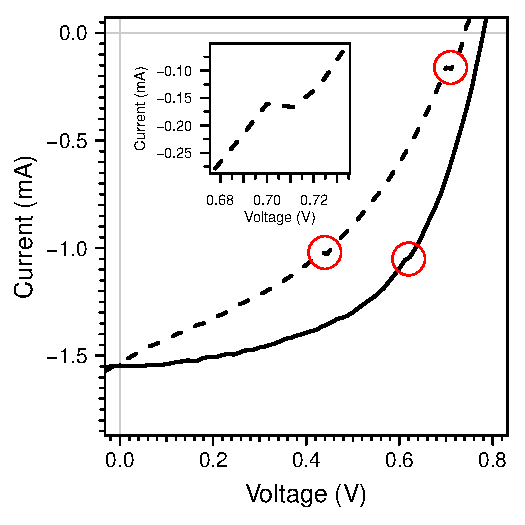
\includegraphics[width=0.5\textwidth]{autoscale/ig1-3-1-int4.pdf}
	\mycaption[Kinks in JV sweep due to autoscale.]{A current-voltage sweep of an hysteretic perovskite solar cell with Keithley autoscale active. Both the forward (dashed) and the reverse (solid line) present small discontinuities around \SI{1}{\mA} and \SI{0.1}{\mA}.}\label{fig:autoscale}
\end{SCfigure}

In literature one can easily find current-voltage curves with discontinuities and kinks\cite{Li2016,Snaith2014,Zhang2015} CITE  10.1039/C4MH00238E  like the one reported in \cref{fig:autoscale}. Some even lucubrate about the origin of these in perovskite solar cells. Indeed this is likely just caused by the auto-scale feature of the Keithley equipment, disabling this, the discontinuities disappears.

\paragraph{Scan speed}
The used sweep speed is \SI{500}{\mV\per\s}, which was arbitrarily chosen for having an aesthetically good looking current-voltage curve (avoiding bumps leading to currents higher than \gls{jsc}), like the one in \cref{fig:iv_ugly}.

\begin{SCfigure}%[!hbtp]%
	\centering
	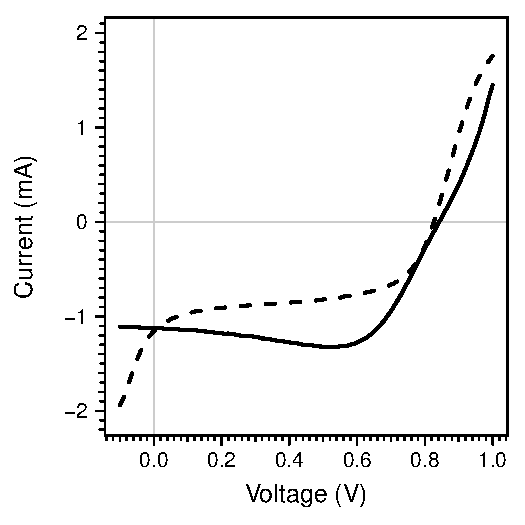
\includegraphics[width=0.5\textwidth]{iv_ugly/ig47-b32-int2-4.pdf}
	\mycaption[Hysteretic current-voltage scan.]{At the employed scan speed, the hysteresis phenomena causes the reverse (solid line) scan to reach currents higher than the \gls{jsc}.}\label{fig:iv_ugly}
\end{SCfigure}

Due to hysteresis phenomena, no scan speed, direction, or precondition is the correct one and they all heavily affect the resulting \gls{pce}. Indeed has been shown that even so-called "hysteresis-free" perovskite solar cells can have hysteresis on smaller or bigger time scale\cite{Jacobs2018}. Rather, a static measurement or a \acr{mppt} should be used for obtaining a result not completely alienated from the real world.

The noise often observed in current-voltage scans at high sweep speeds is mainly caused by oscillations in the solar simulator illumination intensity, as an example see REFERENCE FIGURE. Indeed, using a white \gls{led} as illumination source, this noise is not present but the spectral mismatch affects the meaningfulness of the measurement.

\paragraph{Stabilized or dynamic current-voltage sweeps}
One very appealing alternative to current-voltage sweeps are the so-called "stabilized current-voltage sweeps", where at each voltage point a fixed stabilization time is waited and the stabilised current is reported. CITE 10.1039/c4ee02465f 10.3390/photonics2041101
An improvement of this technique is named "dynamic current-voltage sweeps", here the stabilization step is of variable duration, until the current-time derivative falls below a threshold (e.g. \SI{0.2}{\%\per\minute}).CITE 10.1039/c7ta05609e 10.1002/pip.2839
In this thesis, these techniques have not been used.

\paragraph{Shunt and series resistances} \label{resistances} In our group the shunt and series resistances are evaluated by the current versus voltage derivative of a dark current-voltage sweep respectively at zero and at high-enough voltage. This methodology is inherited from organic solar cells and, as is easy to foresee, is unreliable on hysteretic devices: in the case of perovskite solar cells a measurement of the stabilised current at a few points have better chances to produce a useful result. The measurement of the current at a voltage close to zero is enough for estimating the shunt resistance while two points at high voltages are needed for estimating the series resistance.

\section{\textsmaller{V\textsubscript{OC}} and \textsmaller{J\textsubscript{SC}} Dependence on Light Intensity}
The illumination by solar simulation is reduced via neutral density filters with transmittance of 0.05, 0.12, 0.25, 0.51, 0.81 and 1 (no filter). The devices are kept at this reduced illumination $\phi$ and at open circuit or short circuit conditions until steady state for measuring respectively $V_{OC}(\phi)$ or $J_{SC}(\phi)$.

\paragraph{\Gls{jsc} versus $\phi$}\label{methods_jsc_intensity} The \gls{jsc} dependency on the light intensity $\phi$ can be fitted with a power law $J_{SC} \propto \phi^\alpha$ giving $\alpha$ values usually from 0.95 to 1.

\paragraph{\Gls{voc} versus $\phi$}\label{methods_voc_intensity} The \gls{voc} dependency on the light intensity $\phi$ can be fitted with a natural logarithmic (the base of the logarithm comes from Boltzmann distribution) dependence as:
$$V_{OC} = k + \frac{n_{id} k_B T}{q}\cdot\ln(\phi)$$
where $k$ does not contain physical meaning (depends on the light intensity units and on the \gls{voc} at 1~sun), $k_B$ is Boltzmann constant, $T$ is temperature in Kelvin, and $q$ is the elementary charge\cite{Calado2018b} (in literature one can found inexact reports of ideality factor determined via \gls{voc} versus \gls{jsc} dependency). The so-obtained ideality factor $n_{id}$ is usually from 1 to 2. In this thesis, this measurement is reported both from static measurement of \gls{voc} (proper method) and from \gls{voc} obtained from current-voltage sweeps; the used method is specified case by case.	An applied voltage dependent ideality factor can also be measured from a current-voltage sweeps in dark but has not been evaluated in this thesis. Anyway in perovskite solar cells exhibiting hysteresis, a current-voltage sweep would not give fair ideality factors and the current-voltage points should be acquired reaching steady state conditions for each point. Both these methods for deriving the ideality factor have been implemented in the DrIFtFUSION simulation as described in \cpageref{dd_ideality}.

For the interpretation of these results, see \cpageref{interpretation_lightintensity}.

\section{Charge Extraction (\textsmaller{CE})}

The device is kept under 1~sun equivalent illumination by a white \gls{led} at open circuit conditions until stabilization is reached. 1~sun equivalent illumination is defined as the illumination at which the a silicon photodiode gives the same \gls{jsc} as under calibrated 1~sun from the solar simulator. The \gls{led}-solar spectral mismatch affects slightly the measurement, but in no case a \gls{pce} is reported from any \gls{led}-illuminated experiment. After stabilization the illumination is switched off and, at the exactly same moment, the device is short circuited through a small and known resistance of \SI{50}{\ohm} \cite{Duffy2000}.

This is repeated decreasing the light intensity from 1~sun down to dark (in dark no signal should be observed, indeed some residual charge can usually be seen, the reason of this could be ionic profile updating or an insufficient darkness) and a single decay is measured for each illumination point, over approximatively 30 illumination points.

The equipment includes two transistors (in a in-house built circuit by Javier Pérez Hernández) connected to a pulse generator providing a square pulse long at least as the measurement window. I suggest to reduce as much as possible the duration of the dark period (ruled by the pulse generator) in order to save time for the stabilization step in the next measure.

The measurement is carried out with an oscilloscope in parallel to the known small resistance. In the first microseconds, most of the free charge flows through the resistor generating a voltage drop across it which is measured by the oscilloscope. This potential drop can be converted to current using the Ohm's law, which, integrated over time, gives the amount of extracted charge.

For the interpretation, see \cpageref{interpretation_ce}; for the implementation, see \cpageref{r_ce}.

\paragraph{Noise reduction}\label{r_ce_noise}
Most of the observed short-times noise (\SI{< 5E-7}{\s}) is, supposedly, related to the opening and closing of the transistors included in the in-house built circuit.

Annoyingly, the noise profile is characteristic of the cell and of the circuitry, so a simple average over many decays does not help in cancelling it.

This affects the resulting measurement to a noticeable extent, which starts to be a problem if the charge versus light bias (\gls{voc} generated at a given illumination intensity) profile has to be studied in detail, as in \cref{ch:tae}.

In order to reduce this effect various approaches have been tested; finally the single decays were fitted with a bi-exponential formula (sum of two exponential) and the integral of this fit was used.

\section{Transient PhotoVoltage (\textsmaller{TPV})}
\epigraph{\textit{"Imma firin mah lazor\\pewpew pewpewpew"}}

The device is kept under 1~sun illumination by a white \gls{led} ring at open circuit until stabilization is reached. 1~sun equivalent illumination is defined as the illumination at which the a silicon photodiode gives the same \gls{jsc} as under calibrated 1~sun from the solar simulator. Then an additional illumination pulse is provided by a nitrogen laser. The pulse duration is around \SI{1.5}{\ns}. The equipment can output up to 20~pulses per second, but due to the oscilloscope settings and oscilloscope internal memory speed we're limited to 1~pulse per second (maybe decreasing the number of acquired points would allow us to acquire higher repetition rates). The pulse was triggered with a square wave pulse generator. The wavelength is selected with the absorption and emission of a dissolved molecular dye, usually a wavelength of \SI{650}{\nm} is selected using a RhodamineB solution\cite{RadiantDyesLaser}, this wavelength allow us to illuminate in deep the perovskite layer (in contrast to a blue light where the illumination would be absorbed within the first hundreds of nanometres of the material).

During all the process, the device is connected to a \SI{1}{\Mohm} oscilloscope, registering the open circuit voltage profile (the high resistance of the oscilloscope is a good approximation of open circuit). An auxiliary output from the square wave pulse generator used for the pulse is used for the trigger of the oscilloscope.

The intensity of the laser pulse is decreased using a variable neutral density filter (a partially reflecting wheel with different positions for different transmittivities) so that the voltage perturbation caused by the light pulse does not exceed \SI{10}{\mV} with 1~sun background illumination intensity. We consider this as a "small-enough" perturbation.

This process is repeated decreasing the light intensity from 1~sun down to dark. Clearly, the pulse intensity which could be considered a "small-enough" perturbation at high background illumination is not so at lower ones and cannot be small at dark conditions. We \emph{do not} regulate the pulse intensity depending from the background illumination for being able to use this data also for \acr{dc} studies. The \acr{dc} does not intrinsically need the usage of a constant pulse intensity but it needs the measurement of a \acr{tpc} for each pulse intensity. The switch from \acr{tpv} to \acr{tpc} setups and back would be complex and time demanding with the current setup. Anyway quite all the information from the \acr{tpv} is obtained from the high background illumination intensity measurements.

For each illumination intensity, the reported decay is the result of averaging around 30~transients. This manages to reduce the noise.

For the interpretation, see \cpageref{interpretation_tpv}; for the implementation, see \cpageref{r_tpv}.


\paragraph{Noise treatment}\label{tpv_robust}

Most of the observed noise (\SI{< 2E-7}{\s}) is due to the radiofrequency emitted by the spark in the nitrogen laser which gets absorbed by all the non-coaxial cables (coaxial ones don't) and from the circuitry of the samples holder acting as a receiving antenna. On the contrary to what happens for \acr{ce}, the short times noise seems to not follow a constant pattern, so averaging the measurement over a few repetitions (usually 30) manages to reduce the noise.

This noise can affect the exponential or bi-exponential fitting, for this reason a robust fitting routine has been used, which gives a lower weight to outlier points. An example can be seen in \cref{fig:tpv_robust}.

\begin{figure}
	\centering
	\includegraphics[width=0.9\textwidth]{{tpv_robust/TPV_ig52-68-3_0.883897_V-monoexp}.pdf}
	\mycaption[Robust and normal fitting comparison.]{In grey the fitted points, in yellow the points not considered for the fitting, the solid black line is the \gls{loess}. The normal non-linear least squares fitting (in green) is affected by noise, outliers and characteristics not of interest by the model. The non-linear robust fitting (in brown) manages to reduce the weight of these points.}\label{fig:tpv_robust}
\end{figure}


\paragraph{Voltage Increase Value}\label{tpv_deltaV}

The value of the voltage increase due to the additional illumination is needed for \acr{dc} measurement.

In the group this $\Delta V$ value was traditionally obtained subtracting the steady state \gls{voc} from the maximum voltage point in the measured transient. This is obviously heavily affected by the aforementioned noise when a short time window is used.

The following alternatives were tested:
\begin{itemize}
	\item The linear factor in an exponential fit was used, but it can fail if the decay does not have a simple exponential shape (often a bi-exponential, sum of two exponentials, is observed);
	\item The sum of the two linear factors in a bi-exponential fit, which could work but one have to carefully set boundary values to the fitting parameters for avoiding a fast exponential matching just some noise;
	\item The maximum value of a \gls{loess} local regression was used, but this underestimates the value, especially when the peak top are just few points (when the measurement time window is large);
	\item The average of the values registered starting from the maximum voltage point and during a specified time lapse.
\end{itemize}

This last option is the one currently in place. The average was performed over \SI{50}{ns} after the peak and this allowed us to get a reliable $\Delta V$ value.

\section{Transient PhotoCurrent (\textsmaller{TPC})}

The device is kept under 1~sun illumination by a white \gls{led} ring at short circuited through a \SI{50}{\ohm} resistor until stabilization is reached. 1~sun equivalent illumination is defined as the illumination at which the a silicon photodiode gives the same \gls{jsc} as under calibrated 1~sun from the solar simulator. Then an additional illumination pulse is provided by a nitrogen laser.

The signal is acquired by an oscilloscope in parallel to the \SI{50}{\ohm} resistor. This allows us to measure a potential drop across the resistor and the related current via Ohm's law. Subtracting the constant current due to the background illumination and integrating the transient over time gives the charge generated by the laser pulse.

This process is repeated at 1~sun and at dark background illumination conditions.

For each illumination intensity, the reported decay is the result of averaging around 30~transients. This manages to reduce the noise.

For the interpretation, see \cpageref{interpretation_tpc}; for the implementation, see \cpageref{r_tpc}.

\section{Differential Capacitance (\textsmaller{DC})}

This is a meta-measurement as it just combines the data from \acr{tpv} and \acr{tpc} without requiring any additional experiment\cite{Shuttle2008}, sometimes also referred to as "differential capacitance".

As explained in \cpageref{interpretation_dc}, the electrical capacitance of a solar cell is not a constant (as in most of the commercial capacitors), indeed it depends on the applied voltage bias or light bias.

The charge obtained with the \acr{tpc} (in case the dark and illuminated results were different, the third quartile of all \acr{tpc} measurements was used) is divided by an array of values obtained from \acr{tpv}, one for each illumination intensity. The needed value is the \gls{voc} increase due to the laser pulse, prior to the decay to steady state, for each illumination intensity (obtained as described in \cpageref{tpv_deltaV}).

This allows us to estimate the capacitance of the solar cell device at open circuit with various illumination intensities.

For the interpretation, see \cpageref{interpretation_tpc}; for the implementation, see \cpageref{r_tpc}.


\section{Time-Resolved PhotoLuminescence}
influence of pulse intensity CITE https://arxiv.org/abs/1805.00263
PL wile applying voltage sweep shows hysteresis 10.1021/acs.jpcc.7b06711

Petrozza CITE 10.1021/acsenergylett.6b00355


\section{Impedance Spectroscopy}

\section{Stark Spectroscopy (ElectroAbsorbance)}

\section{Our Solar Cells Characterization Steps}

In this section I'll describe the routinary characterization performed in Palomares group.


